\chapter{Proposed Method}
\label{sec:proposed}
In this section, the discussion centers on the proposed method which improves the problems described in Sec.\ref{sec:problems}.
First, the $L_{2}$ - $L_{p}$ variational retinex model which further considers the feature of the reflectance and illumination is introduced in Sec. \ref{sec:L2-LP}. 
Second, adaptive texture map which adaptively constraint noise amplification in dark regions and over-enhancement in bright regions is described in Sec. \ref{sec:adaptive}. 
Finally, the effectiveness of the proposed method is shown in comparison with the related work by using the output of some images in Sec. \ref{sec:analysis}.\par
Fig. \ref{fig:proposed/flowchart} shows the flowchart of the proposed method.
To explain the flow of the proposed method briefly, the proposed method obtains a low-light image and the initialized illumination which is called the bright channel prior. Next, the proposed method converses a low-light image to HSV-Color scale and extract only value (V) channel. The proposed method iteratively solves the sub-problems related with the reflectance and illumination and gets their component which meet the constraints are appropriate for each component. Finally, the proposed method multiply the estimate reflectance and illumination, converses the obtained enhanced image to RGB-Color space.

%----提案手法のフローチャート---- %
\begin{figure}[htbp]
	\centering
	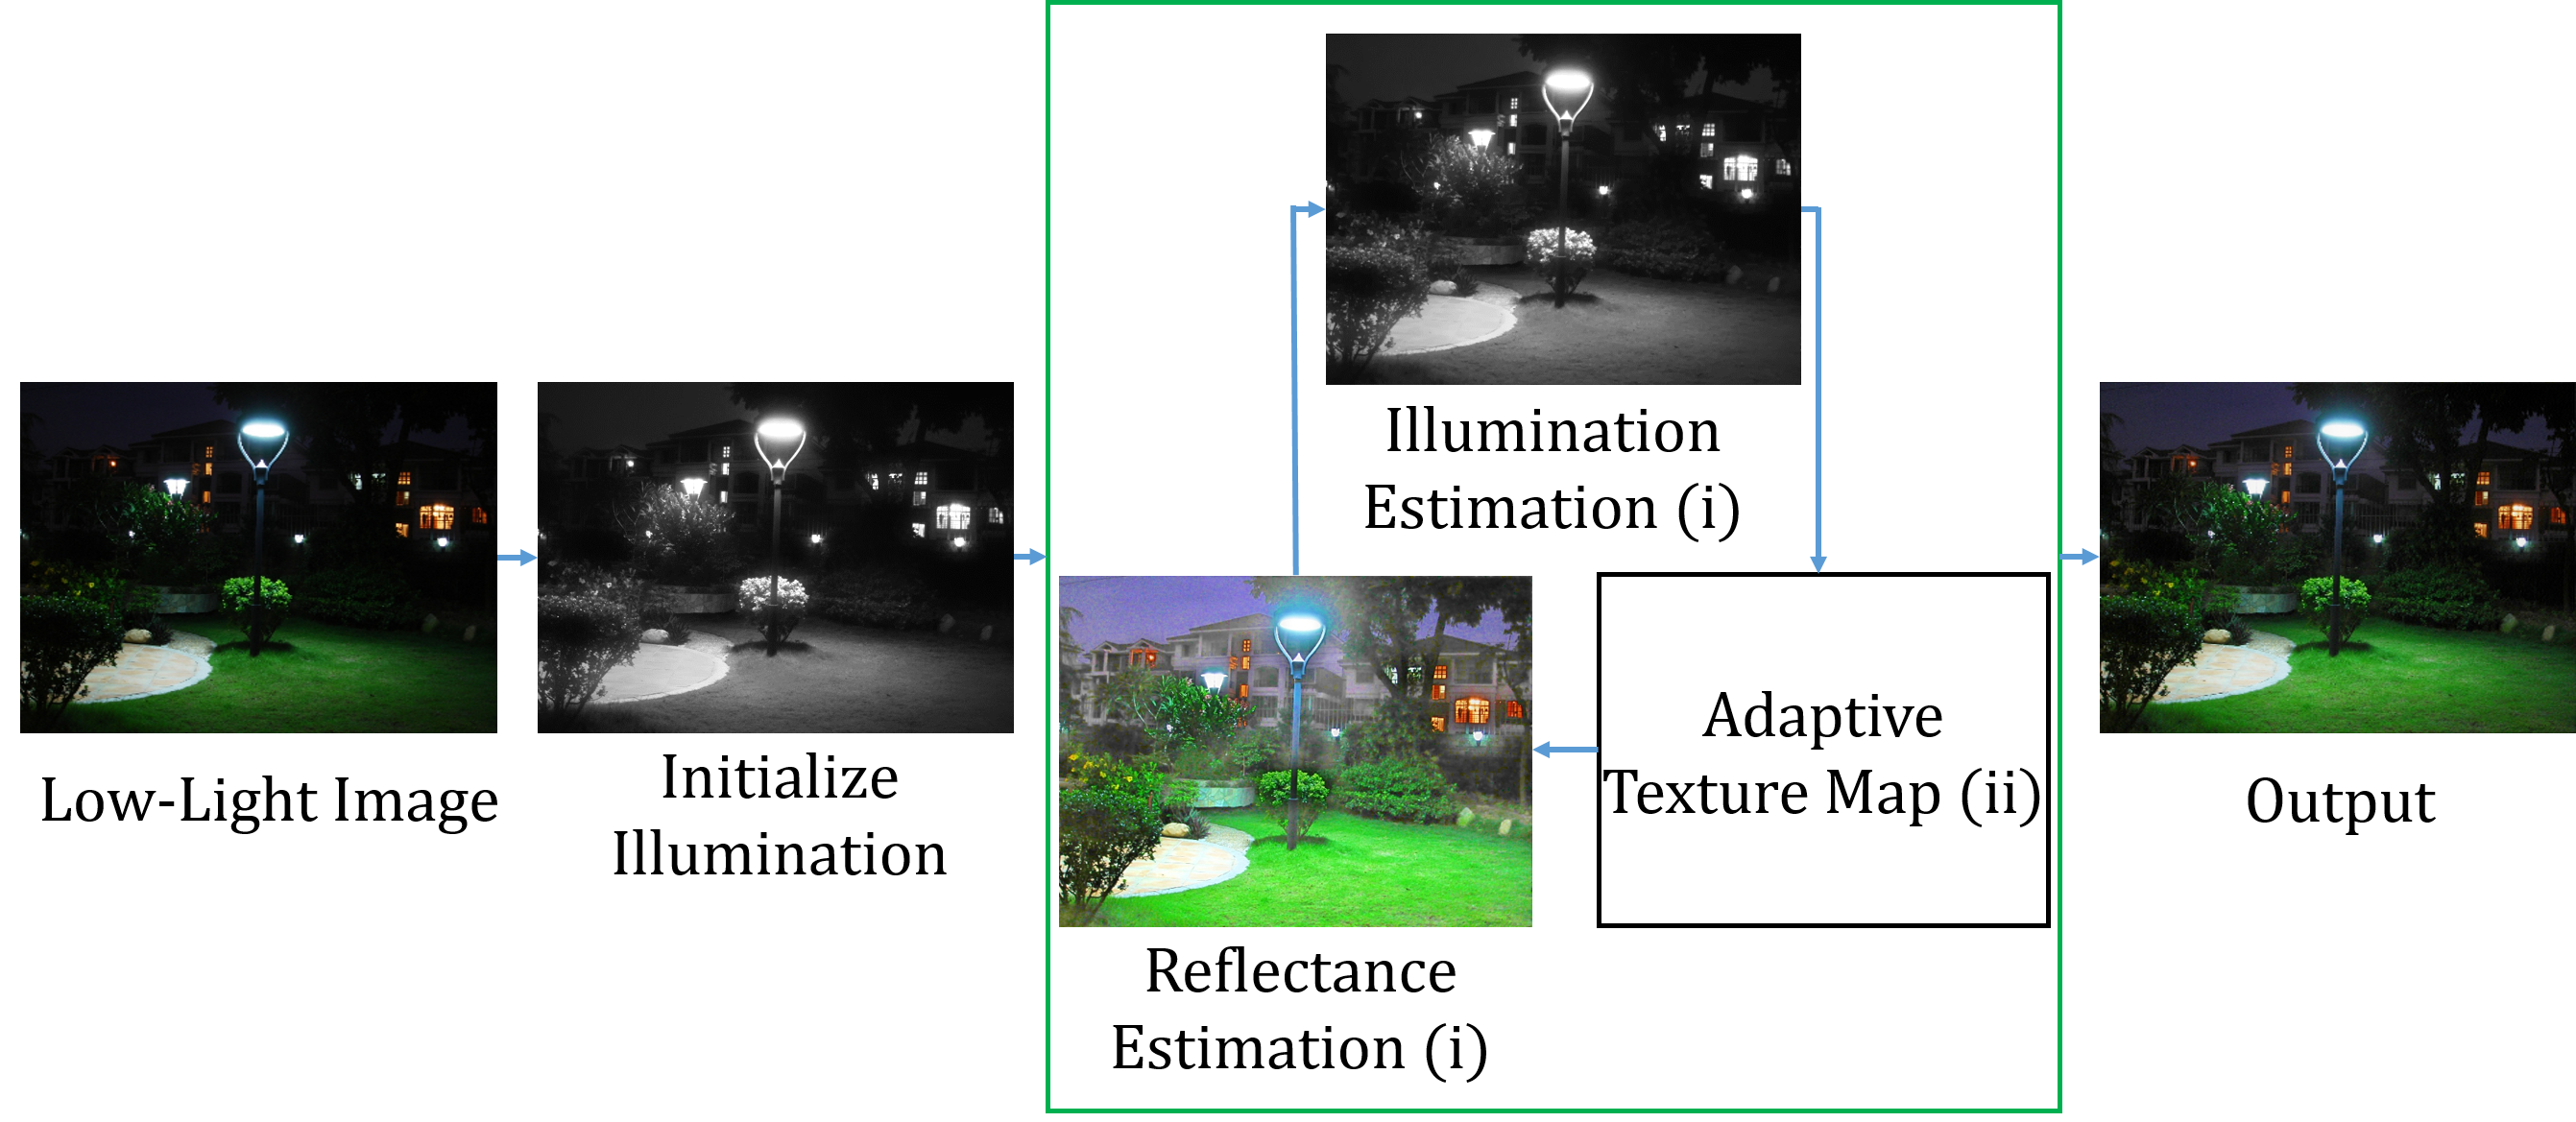
\includegraphics[width=1.0\hsize]{images/proposed/flowchart.eps}
	\caption{The image represents the flowchart of the proposed method. (i)The proposed method changes the constraint terms further considered the characteristics for each component. (ii)The proposed method generates adaptive texture map to constrain noise  amplification and over-enhancement in the estimated reflectance. } \label{fig:proposed/flowchart}
\end{figure}

\section{L2-LP Variational Model} \label{sec:L2-LP}
The conventional methods adopt the $L_{1}$ norm to the constraint term on the reflectance, but the fine detail of the estimated reflectance are susceptible to be damaged. Furthermore, by adopting the $L_{2}$ norm to the constraint term on the illumination, the estimated illumination over-smooths and loss the structure information. Therefore, the proposed method adopts $L_{2}$ - $L_{P}$ norm regularization to each constraint term in order to estimate the reflectance as much as possible to preserve tiny details and estimate the illumination as much as possible to keep the structure information while removing texture component.
The new joint optimization equation is given as:
\begin{equation}
E(I, R) = \argmin_{R, I} \|R \circ I - S\|_{2}^{2} + \alpha \left \|\frac{\nabla{I}}{\frac{1}{\Omega}\Sigma_{\Omega}\nabla{I}+\epsilon}\right\|_{p}^{p} + \beta \|W \circ \nabla{R}\|_{2}^{2} + \gamma \|I - B\|_{2}^{2}, \label{eq:proposed/equation}
\end{equation}
where $\| \cdot \|_{p}$ denotes the $L_{p}$ norm regularization term $(0 < p \leq 2)$, and $W$ is adaptive texture map related to the reflectance $R$. As described in \cite{l2-lp}, a block coordinate descent \cite{block} is used in order to find an optimal solution to the non-convex objective function $(\ref{eq:proposed/equation})$. Since the $L_{p}$ regularization term causes non-smooth optimization, the proposed method adopts an iteratively re-weighted least square (IRLS) method \cite{iterate} and rewrite the second term in $(\ref{eq:proposed/equation})$ as:
\begin{equation}
\left \|\frac{\nabla{I}}{\frac{1}{\Omega}\Sigma_{\Omega}\nabla{I}+\epsilon}\right\|^{p} = \|U \circ \nabla{I}\|^{2}, \label{eq:approximation}
\end{equation}

\begin{align}
U &= \left \{
	\begin{array}{ll}
	\frac{1}{\xi^{2-p}}, 
	& \left |\frac{\nabla{I}}{\frac{1}{|\Omega|} \sum_{\Omega} \nabla{I} } \right| < \xi\\
	\frac{\left |\Sigma_{\Omega} \nabla{I} \right|^{2-p}}{\left |\nabla{I} \right|^{2-p}} \frac{1}{\left |\Sigma_{\Omega} \nabla{I} \right|^{2}},
	& \rm{otherwise}
	\end{array}
\right.\\
  &= \left \{
  	\begin{array}{ll}
  	\frac{1}{\xi^{2-p}}, 
  	& \left |\frac{\nabla{I}}{\frac{1}{|\Omega|} \sum_{\Omega} \nabla{I} } \right| < \xi\\
  	\frac{1}{\left |\Sigma_{\Omega} \nabla{I} \right|^{p} \left |\nabla{I} \right|^{2-p}},
  	& \rm{otherwise}
  	\end{array}
\right. \label{eq:lp_shape}
\end{align}
where the variable $u$ is only approximate variable. This is because the Eq. \ref{eq:approximation} uses a $L_{2}$ norm format $\Phi(\frac{\nabla{I}}{\frac{1}{\Omega}\Sigma_{\Omega}\nabla{I}+\epsilon};\xi)$ based on \cite{l0-sparse} to approximate the $L_{0} $ norm function. As can be seen in Fig. \ref{fig:nom_p/comparison}, the red curve can approximate the most sparse $L_{0}$ function. Therefore, the proposed method can remove fine textures and preserve meaningful salient structures in the estimated illumination. As shown in Fig. \ref{fig:nom_p/graph_norm_p}, with the decease of the value $\xi$, the $L_{p}$ norm function is getting close to the $L_{0}$ function. Therefore, large-$\xi$ are more convex-like and easy to optimize, in contrast, small-$\xi$ are more steep and difficult to optimize.\par
Fig. \ref{fig:comparison_p} shows the effect of changing the value of $p$ in the range ($0 < p \leq 2$) in the estimated illumination. As the value of $p$ decreases, the estimated illumination leaves smooth and texture-less. Concomitantly, the estimated reflectance contains more rich textures and details. In particular, when $p=0$, some salient structure information in the estimated illumination may be lost too much, because the $L_{0}$ norm has strong sparsity. 
%----Lpノルムの概形----
\begin{figure}[t]
\vspace{-15pt}
	\begin{minipage}[b]{0.5\hsize}
		\centering
		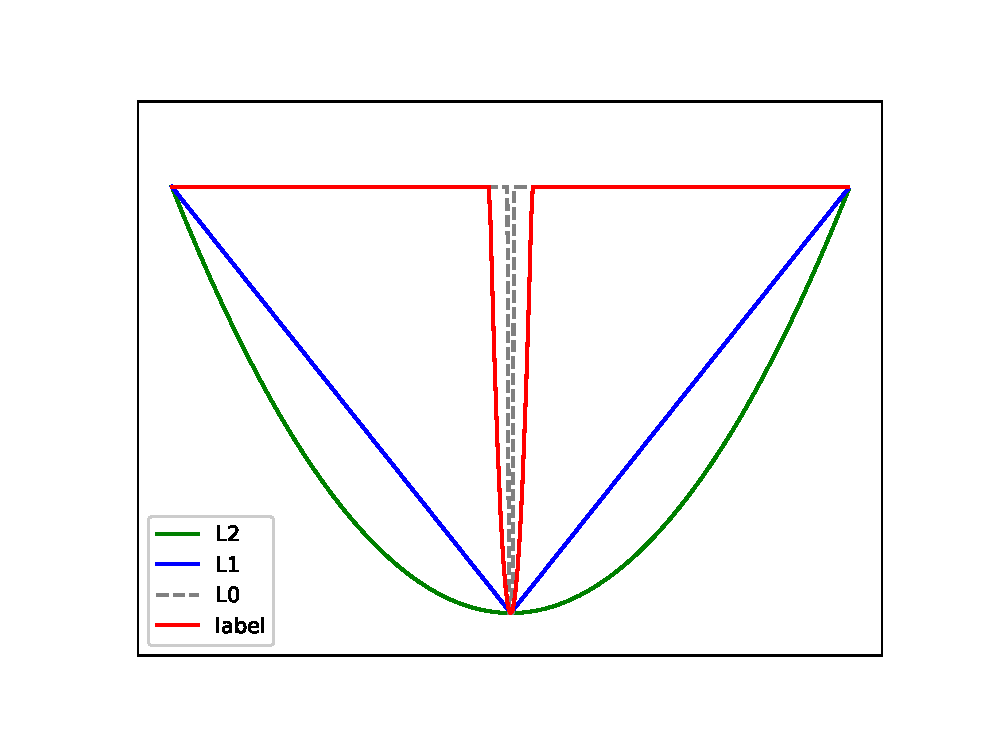
\includegraphics[width=64mm, height = 48mm]{images/norm_p/graph/graph_norm.eps}
		\subcaption{Plots of different penalty functions} \label{fig:nom_p/comparison}
	\end{minipage}
	\begin{minipage}[b]{0.5\hsize}
		\centering
		\includegraphics[width=64mm, height = 48mm]{images/norm_p/graph/graph_norm_p.eps}
		\subcaption{Plots of $L_{p}$ norm for different values $p$} \label{fig:nom_p/graph_norm_p}
	\end{minipage}
	\caption{The images represent various plots about the $L_{p}$ norm.}
	\label{fig:graph_lp}
\end{figure}
%----ノルムpによる推定比較---- %
\begin{figure*}[htbp]
\centering
	\begin{minipage}[b]{0.32\hsize}
	\centering
	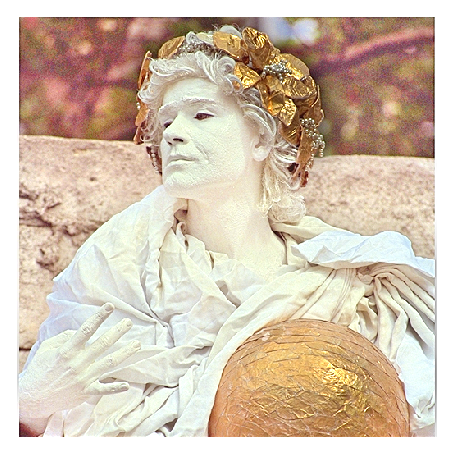
\includegraphics[width=49mm, height = 49mm]{images/norm_p/reflectance/p06.eps}
	\end{minipage}
	\begin{minipage}[b]{0.32\hsize}
	\centering
	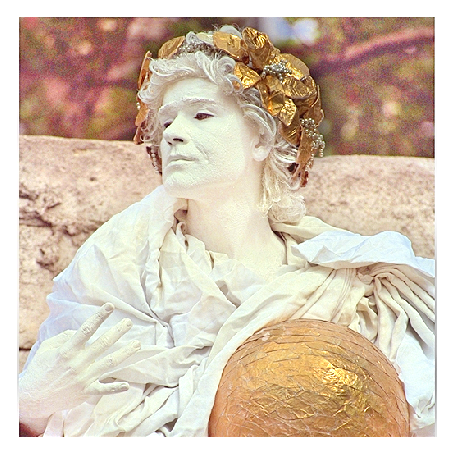
\includegraphics[width=49mm, height = 49mm]{images/norm_p/reflectance/p10.eps}
	\end{minipage}
	\begin{minipage}[b]{0.32\hsize}
	\centering
	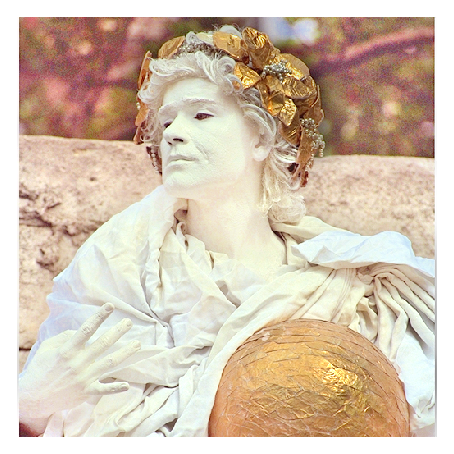
\includegraphics[width=49mm, height = 49mm]{images/norm_p/reflectance/p20.eps}
	\end{minipage}\\
	\vspace{1.5mm}
	\begin{minipage}[b]{0.32\hsize}
	\centering
	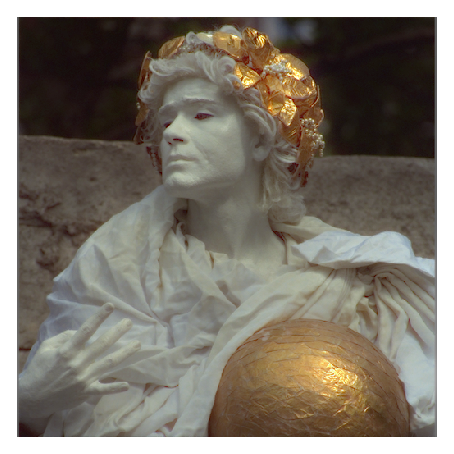
\includegraphics[width=49mm, height = 49mm]{images/norm_p/illumination/p06.eps}
	\subcaption{$p$=0.6} \label{fig. p-04}
	\end{minipage}
	\begin{minipage}[b]{0.32\hsize}
	\centering
	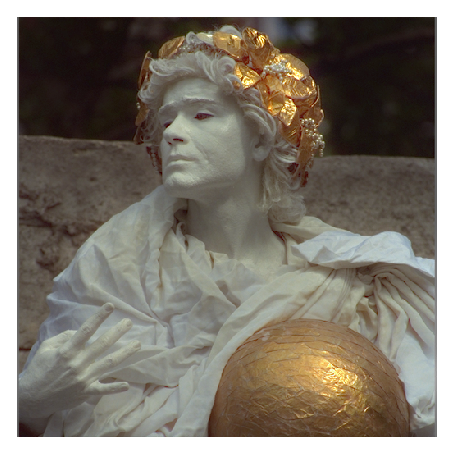
\includegraphics[width=49mm, height = 49mm]{images/norm_p/illumination/p10.eps}
	\subcaption{$p$=1.0} \label{fig. p-10}
	\end{minipage}
	\begin{minipage}[b]{0.32\hsize}
	\centering
	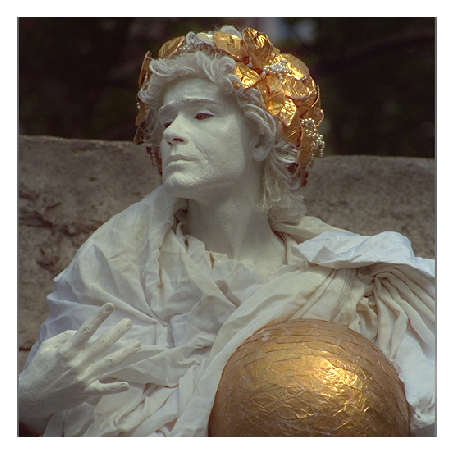
\includegraphics[width=49mm, height = 49mm]{images/norm_p/illumination/p20.eps}
	\subcaption{$p$=2.0} \label{fig. p-20}
	\end{minipage}
	\caption{Comparison of decomposition results for different values of norm $p$. ((a)-(c) top: reflectance, bottom: illumination)}
	\label{fig:comparison_p}
\end{figure*}
\section{Adaptive Texture Map} \label{sec:adaptive}
Low-light images usually have much noise hidden in dark regions. However, noise reduction over the entire images can damage detail in bright regions. In addition, the preferable reflectance's gradients should be smooth in homogeneous regions while undamaged at edges. 
Therefore, $W$ is set so that the third term performs strong noise reduction in dark and homogeneous regions, while it performs weak noise reduction in bright and textures regions. The formulation of $W$ is given as:
\begin{equation}
W_{d} = W_{B} \circ A_{d}, \label{eq: adaptive_texture}
\end{equation}
where $d$ represents horizontal ($h$) and vertical ($v$) directions, and $W_{B}$ represents the initial estimated weight map by inverting the normalized bright channel, and $A_{d}$ represents the texture map that effectively distinguish between homogeneous and textures regions.\par In the same way as in \cite{activation}, $W_{B}$ is chosen to selectively assign different weight values to both bright and dark regions:
\begin{equation}
W_{B} = 1.0 - \max_{c \in \{r, g, b\}}S^{c}. \label{eq: initial_weight}
\end{equation}
\par
Furthermore, texture map is set as the inverse of the $a_{r}$-th power of the absolute value of a mean local variation (MLV) \cite{jiep} that can significantly distinguish between homogeneous regions and textures regions:
\begin{equation}
A_{d} = \frac{1}{\left |\frac{1}{|\Omega|}\sum_{\Omega}\nabla_{d}{R} \right|^{a_{r}} + \epsilon}, \label{eq: mlv}
\end{equation}
where $a_{r} (< 1)$ is an exponential parameter to adjust the texture awareness for the reflectance. 
Figure \ref{fig:mlv_pow} shows that tiny details are more revealing, as the value of $a_{r}$ decreases exponentially. Furthermore, the MLV of the reflectance can extract more rich gradient information than that of an observed image. Thus, by inverting the $a_{r}$-th power of the MLV of the reflectance, $A_{d}$ can adaptively assign a small value in textures regions and a large value in homogeneous regions. 
Comparing Fig. \ref{fig:wo} and \ref{fig:w}, we see that the estimated reflectance with $W$ can suppress over-enhancement in bright regions and noise amplification in dark regions. Moreover, the estimated reflectance with $W$ can reveal details and textures in spite of noise reduction. 
\begin{figure}[t]
\centering
\begin{minipage}[b]{0.32\hsize}
\centering
\includegraphics[height=0.75\hsize]{images/noise/input.eps}
\subcaption{Observed image} \label{fig:weight_input}
\end{minipage}
\begin{minipage}[b]{0.32\hsize}
\centering
\includegraphics[height=0.75\hsize]{images/noise/MLV_10.eps}
\subcaption{MLV ($a_{r}=1.0$)} \label{fig:mlv_normal}
\end{minipage}
\begin{minipage}[b]{0.32\hsize}
\centering
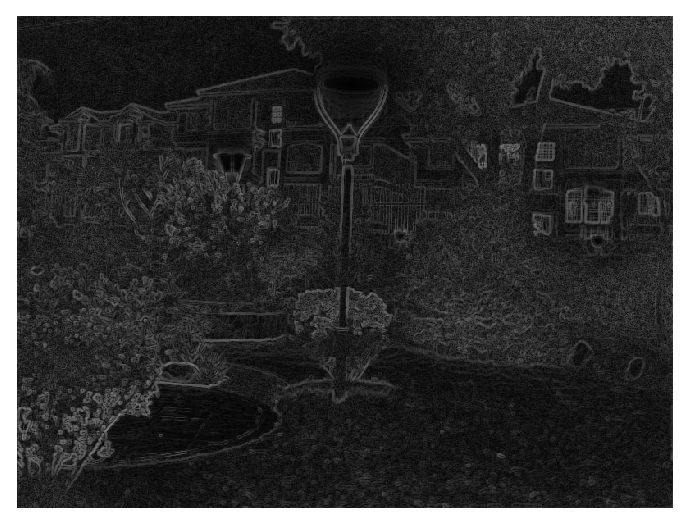
\includegraphics[height=0.75\hsize]{images/noise/MLV_05.eps}
\subcaption{MLV ($a_{r}=0.5$)} \label{fig:mlv_pow}
\end{minipage}
\caption{Comparison of MLV results for different values of $a_{r}$. As the value of $a_{r}$ decreases, MLV can obtain more rich gradient information.}
\label{fig:mlv_change}
\end{figure}

\begin{figure}[t]
\centering
\begin{minipage}[b]{0.49\hsize}
\centering
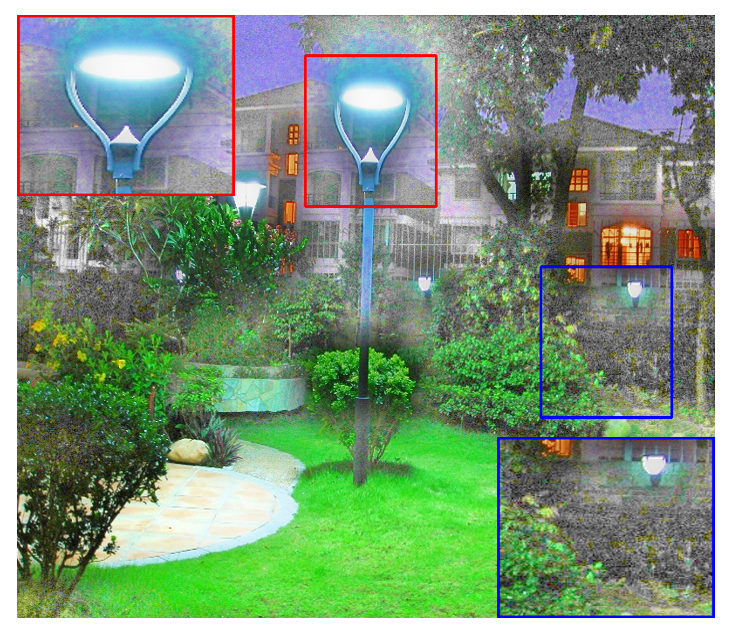
\includegraphics[width = 48mm, height=36mm]{images/noise/mlv_wo.eps}
\subcaption{Reflectance w/o $W$} \label{fig: wo}
\end{minipage}
\begin{minipage}[b]{0.49\hsize}
\centering
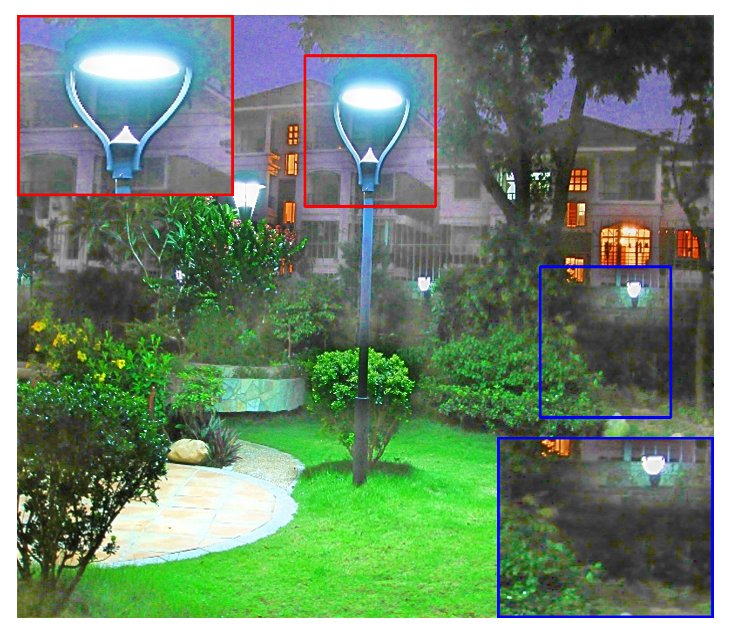
\includegraphics[width = 48mm, height=36mm]{images/noise/mlv_reflectance.eps}
\subcaption{Reflectance with $W$} \label{fig: w}
\end{minipage}
\caption{Comparison of reflectance results. (a) the estimated reflectance without $W$; (b) the estimated reflectance with $W$.}
\label{fig: noise_suppression}
\end{figure}

\section{Solution} \label{sec:solution}
The minimization optimization problem (\ref{eq:proposed/equation}) can be solved by iteratively updating each component. In particular, for the $k$-th iteration of sub-problems.
\begin{enumerate}
\renewcommand{\labelenumi}{\arabic{enumi}).}
\item \textbf{$\boldmath{I}$ sub-problem:} Collecting the terms related to $I$ leads to the following equation (\ref{eq:proposed/equation}):
\begin{equation}
I_{k} = \argmin_{I}\|I \circ R_{k-1} - S\|_{2}^{2} + \alpha\|U \circ \nabla{I}\|_{2}^{2} 
+\lambda \|I - B\|_{2}^{2}. \label{eq: i_subproblem}
\end{equation}
We reduce the equation (\ref{eq: i_subproblem}) to a classic least square problem:
\begin{equation}
i_{k} = \argmin_{i} \|\hat{i}r_{k-1} - s\|_{2}^{2} + \alpha\|\hat{u}Di\|_{2}^{2} + \lambda \|i - b\|_{2}^{2}, \label{eq:classic_i_subproblem}
\end{equation}
where $i$ is the vectorized format of $I$ and $\hat{i}$ represents a diagonal matrix with $i$ as its entries, and $D$ contains $D_{h}$ and $D_{v}$, which are the Toeplitz matrices from the discrete gradient operators with forward difference.
The same notation is used for other matrices (r, s, b corresponds to R, S, and B, respectively). By differentiating equation (\ref{eq:classic_i_subproblem}) with respect to $i$, and setting the derivative to $0$, we have the following solution:
\begin{equation}
i_{k+1} = (\hat{r}_{k-1}^{T}\hat{r}_{k-1} + \alpha D^{T}\hat{u}D + \lambda{1})^{-1} (\hat{r}_{k-1}^{T}s + \lambda{\hat{b}}). \label{eq: i_solution}
\end{equation}
Then, we reformulate the obtained $i_{k}$ into matrix format $I_{k}$.
\item \textbf{$R$ sub-problem:} After acquiring $I_{k}$ from the above solution, the joint optimization (\ref{eq:proposed/equation}) related to $R$ becomes similar to that of $I$:
\begin{equation}
R_{k} = \argmin_{R}\|I_{k} \circ R - S\|_{2}^{2} + \beta\|W \circ \nabla{R}\|_{2}^{2}. \label{eq: r_subproblem}
\end{equation}
In the same way as in the former derivation, we provide the solution of $R$ as follows:
\begin{equation}
r_{k} = (\hat{i}_{k}^{T}\hat{i}_{k} + \beta D^{T}\hat{w}D)^{-1} (\hat{i}_{k}^{T}s). \label{eq: solution_r_subproblem}
\end{equation}
Similarly, we reformulate the obtained $r_{k}$ into matrix format $R_{k}$.
\end{enumerate}
The values of $I$ and $R$ are updated until $\|I_{k}-I_{k-1}\|/\|I_{k-1}\| \leq \varepsilon$ and $\|R_{k}-R_{k-1}\|/\|R_{k-1}\| \leq \varepsilon$ are simultaneously satisfied. After the estimation of  the reflectance and illumination, a Gamma correction operation is adopted to adjust the illumination. Therefore, the final enhanced image is given as $ S_{enhanced} = R \circ I^{\frac{1}{\gamma^{'}}}, \label{eq_final}$ where the empirical parameter $\gamma^{'}$ is set as 2.2. To preserve color information, the Gamma correction is performed in the HSV domain.
\section{Effectiveness of the proposed method} \label{sec:analysis}